\section{Problem 4}
\subsection{Source routing algorithm}

To simplify the notations when describing paths, labels are assigned to paths as shown in Figure \ref{fig:graph}.

\begin{figure}[h]
    \centering
    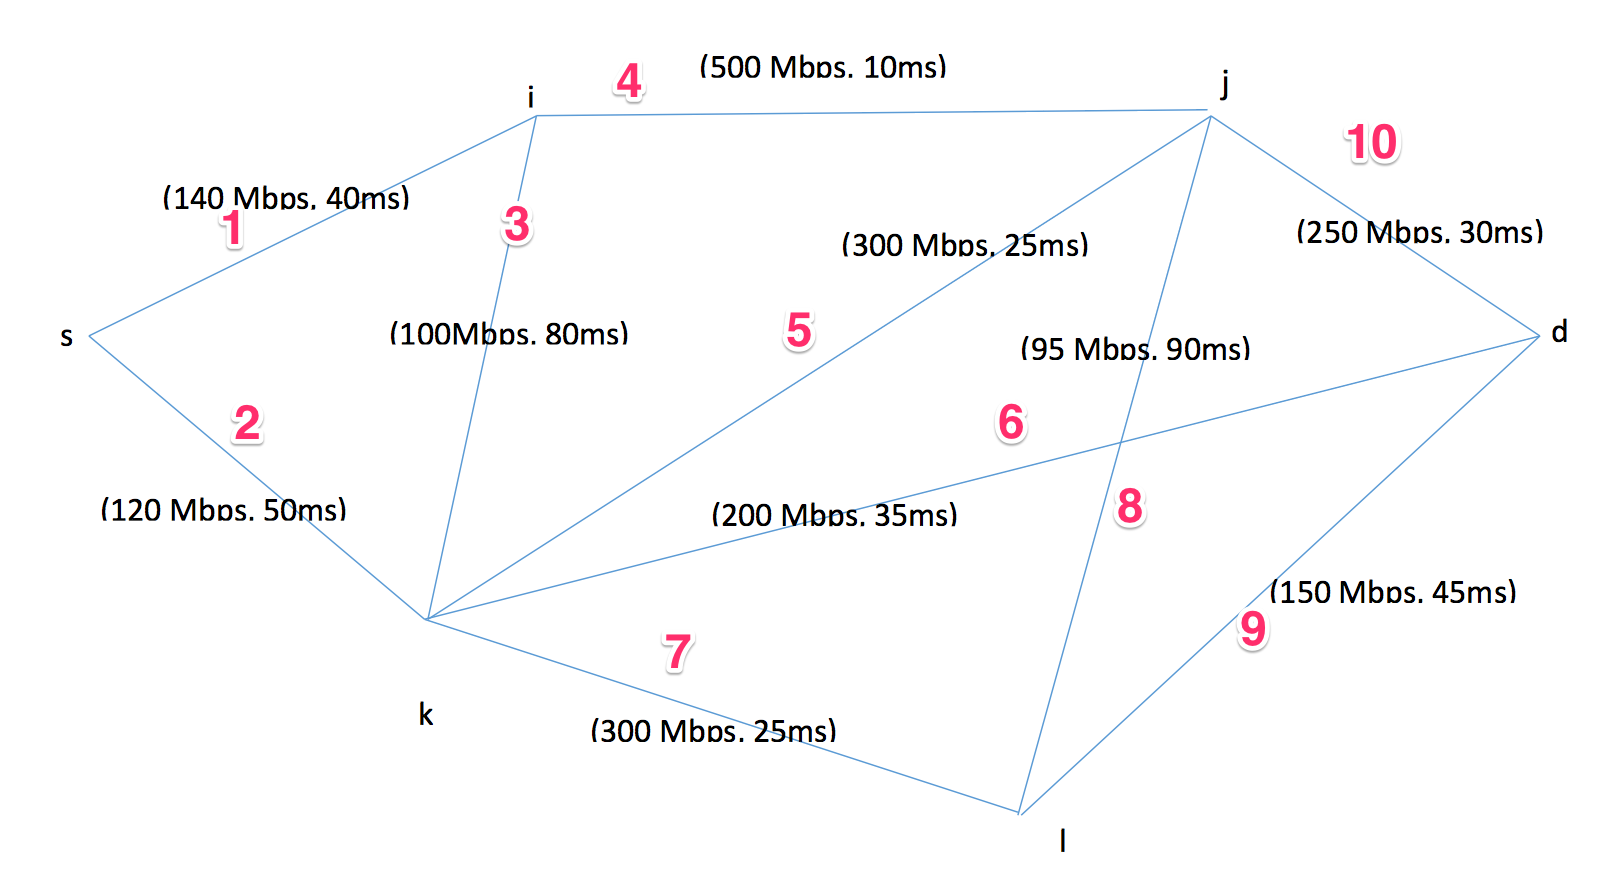
\includegraphics[width=0.8\textwidth]{labeled.png}
    \caption{Graph $G$ with links labeled.}
    \label{fig:graph}
\end{figure}

\textbf{Step 1: generate all paths from s to d that satisfy the bandwidth requirement.}

Noticed that there is only one link, Link 8, in the graph that has a bandwidth under 100Mbs. Therefore, any paths including Link 8 will not satisfy the bandwidth requirement. When generating candidate paths, we exclude those paths which include Link 8. And all other generated paths satisfy the bandwidth requirement.

The paths generated are:
\begin{enumerate}
\item s-1-3-5-10-d
\item s-1-3-6-d
\item s-1-3-7-9-d
\item s-1-4-5-6-d
\item s-1-4-5-7-9-d
\item s-1-4-10-d
\item s-2-3-4-10-d
\item s-2-5-10-d
\item s-2-6-d
\item s-2-7-9-d
\end{enumerate}

\textbf{Step 2: keep paths that satisfy the latency requirement.}

What we do is, for each path listed above, sum up the total latency and exclude those with a total latency higher than 100ms.

The remained paths are:
\begin{enumerate}
\item s-1-4-10-d
\item s-2-6-d
\end{enumerate}

Comparing the delay of these two paths, we see the first path has delay of 80ms and the second one has 85ms. In conclusion, the best path that satisfy both requirements s-i-j-d.


%%%%%%%%%%%%%%%%%%%%%%%%%%%%%%%%
\subsection{Hop-by-Hop routing Algorithm}

The link preference is to choose link with the highest bandwidth. The steps are listed as follows:

\begin{enumerate}
\item Start from origin s.
\item Choose Link 1 over Link 2.
\item Now we reach node i. Choose Link 4 over Link 3.
\item Reach node j.  Link 5 and Link 10 are both valid for the next step.
\item If choose Link 5. Reach node k. Choose Link 7 over Link 6. Reach node l. Choose Link 9 over Link 8. Reach destination d.
\item If choose Link 10. Reach node d.
\end{enumerate}

 Both of these links has the highest bandwidth of 140Mbs. However, the total latency of the first path is 145ms which is greater than second path of 80ms. Therefore, the best path is s-i-j-d.











